%%%%%%%%%%%%%%%%%%%%%%%%%%%%%%%%%%%%%%%%%%%%%%%%%%%%%%%%%%%%%%%%%%%%%%%%%%%%%%%%
\chapter{Συσκευή Καταγραφής Κίνησης}

Στο παρόν κεφάλαιο θα γίνει μια σύντομη ανασκόπηση των χαρακτηριστικών του αισθητήρα. Θα εξηγήσουμε πως δουλεύει ο αλγόριθμος ανίχνευσης του σκελετού που είναι υλοποιημένος εσωτερικά στο \eng{Kinect} και πως μπορούμε να έχουμε πρόσβαση στις τροχιές των αρθρώσεων, που είναι απαραίτητες για να γίνει η καταγραφή της κίνησης. Θα αναφέρουμε εναλλακτικά εργαλεία που μπορεί να χρησιμοποιήσει κανείς και θα κάνουμε μια σύγκριση μεταξύ τους. Τέλος, θα περάσουμε στο κομμάτι των μετρήσεων και των τρόπων βελτίωσης της ποιότητάς τους με την απαλοιφή του θορύβου, που είναι ένα μεγάλο πρόβλημα.

%%%%%%%%%%%%%%%%%%%%%%%%%%%%%%%%%%%%%%%%%%%%%%%%%%%%%%%%%%%%%%%%%%%%%%%%%%%%%%%%
\section{\texorpdfstring{Η Συσκευή \eng{Kinect}}{}}

Ο αισθητήρας της \eng{Microsoft} που πρωτοεμφανίστηκε το 2009 ήταν μια καινοτομία που αρχικά προοριζόταν για την βιομηχανία των παιχνιδιών, αλλά λόγω των πολύ μεγάλων δυνατοτήτων και σχετικά χαμηλής τιμής σύντομα μπήκε στο στόχαστρο της ανοιχτής κοινότητας, η οποία κατάφερε να \lq χακάρει\rq \; και να διαθέσει το πρώτο \eng{API} για πρόσβαση στην συσκευή. Αυτό μετά από λίγο καιρό οδήγησε τη \eng{Microsoft} να διαθέσει το δικό της αντίστοιχο \eng{API}. Το γεγονός που οδήγησε την στροφή των ερευνητών στην χρήση της συσκευής ήταν κυρίως το χαμηλό κόστος, αλλά και οι εκπληκτικές δυνατότητες που παρέχει, καθιστώντας το εύκολο στην χρήση και βολικό για πολλές εφαρμογές.

%%%%%%%%%%%%%%%%%%%%%%%%%%%%%%%%%%%%%%%%%%%%%%%%%%%%%%%%%%%%%%%%%%%%%%%%%%%%%%%%
\subsection{Χαρακτηριστικά}

Το \eng{Kinect} βασίζεται σε τεχνολογία λογισμικού, η οποία αναπτύχθηκε από την εταιρεία \eng{Rare}, θυγατρική της \eng{Microsoft}. Η τεχνολογία της κάμερας ανήκει στην ισραηλινή εταιρεία \eng{PrimeSense}, η οποία ανέπτυξε ένα σύστημα που μπορεί να ερμηνεύσει συγκεκριμένες χειρονομίες, καθιστώντας δυνατό τον έλεγχο ηλεκτρονικών συσκευών χωρίς κάποια άλλη συσκευή εισόδου, παρά μόνο με χειρονομίες σώματος. Για να καταστεί αυτό δυνατό χρησιμοποιείται μια υπέρυθρη κάμερα, ένας προβολέας υπερύθρων και ένα ειδικό μικροτσίπ για την παρακολούθηση της κίνησης των αντικειμένων και των ατόμων σε τρεις διαστάσεις. Αυτό το σύστημα \eng{3D scanner} που ονομάζεται \eng{light coding}, χρησιμοποιεί μια παραλλαγή εικόνας χάρτης βάθους, η οποία μπορεί να αναπαρασταθεί σε τρισδιάστατο χώρο. Η συσκευή διαθέτει μία \eng{RGB} (τρία κανάλια των 8\-\eng{bits}) κάμερα, αισθητήρα βάθους (2048 διακριτές στάθμες -- 11\-\eng{bits}) και \eng{multi-array} μικρόφωνο (Σχήμα \ref{fig:kinect-characteristics}) είναι ικανό να παρέχει πλήρη σωματική απεικόνιση \eng{3D}, καταγραφή κίνησης, αναγνώριση προσώπου και δυνατότητες αναγνώρισης φωνής.

\begin{figure}[H]
    \centering
    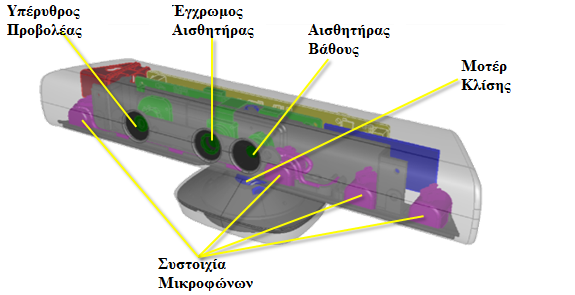
\includegraphics[width=.7\textwidth, height=.2\textheight, keepaspectratio]{fig/kinect-characteristics.png}
    \caption{Δυνατότητες του αισθητήρα \eng{Kinect}\protect\footnotemark}
    \label{fig:kinect-characteristics}
\end{figure}
\footnotetext{Σχήμα από την ιστοσελίδα \eng{\url{http://msdn.microsoft.com/en-us/library/jj131033.aspx}}}

Ο αισθητήρας βάθους αποτελείται από ένα υπέρυθρο προβολέα λέιζερ σε συνδυασμό με ένα μονόχρωμο αισθητήρα \eng{CMOS}, ο οποίος καταγράφει δεδομένα βίντεο σε \eng{3D} κάτω από σχεδόν οποιεσδήποτε συνθήκες φωτισμού. Σύμφωνα με τις πληροφορίες που παρέχονται στους εμπόρους λιανικής πώλησης, το \eng{Kinect} είναι σε θέση να εντοπίζει ταυτόχρονα έως έξι άτομα. Ο χάρτης βάθους που δημιουργείται από τον αισθητήρα βάθους είναι στην ουσία μία εικόνα, η οποία χρησιμοποιεί διαφορετικές αποχρώσεις χρώματος ανάλογα με την απόσταση τον αντικειμένων από την πηγή. Αν αναλογιστεί κανείς το μικρό σχετικά κόστος σε σχέση με τις δυνατότητες και την πληροφορία που παρέχει το \eng{Kinect}, είναι φανερό ότι προσφέρεται για την ανάπτυξη πολύ ενδιαφέροντων εφαρμογών \cite{jean13}. Στον Πίνακα \ref{tab:sensor-characteristics} συνοψίζονται τα βασικά τεχνικά χαρακτηριστικά λειτουργίας.

\begin{center}
    \begin{tabular}{ll}
        \toprule
        % after \\: \hline or \cline{col1-col2} \cline{col3-col4} ...
        \multicolumn{2}{c}{Χαρακτηριστικά} \\
        \midrule
        Ανάλυση & $1280\times 960, \quad 1024\times 768,$ \\
          & $640\times 480, \quad 320\times 240$ \\
        Υπέρυθρη αόρατη δέσμη & $0.4m$ έως $3.5m$ \\
        Χάρτης βάθους, \eng{RGB} ροή δεδομένων & μέχρι 30 \eng{FPS} \\
        Ρύθμιση κάθετης κλίσης & $\pm 27^{o}$ \\
        Κάθετο πεδίο ορατότητας & $43.5^{ο}$ \\
        Οριζόντιο πεδίο ορατότητας & $57^{ο}$ \\
        \bottomrule
    \end{tabular}
    \captionof{table}{Χαρακτηριστικά του αισθητήρα \eng{Kinect}}
    \label{tab:sensor-characteristics}
\end{center}

\begin{figure}[H]
    \centering
    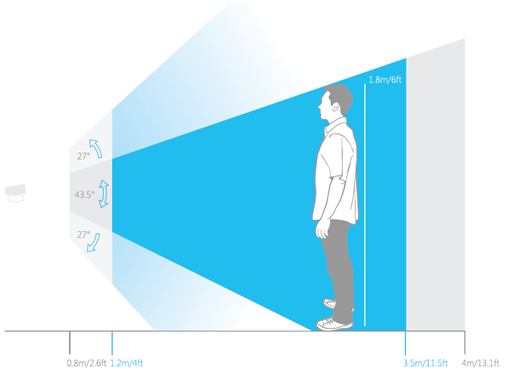
\includegraphics[width=.7\textwidth, height=.35\textheight, keepaspectratio]{fig/kinect-operation-mode.png}
    \caption{Περιγραφή περιοχής λειτουργίας του αισθητήρα\protect\footnotemark}
    \label{fig:kinect-operation-mode}
\end{figure}
\footnotetext{Σχήμα από την ιστοσελίδα \eng{\url{http://msdn.microsoft.com/en-us/library/hh973071.aspx}}}

%%%%%%%%%%%%%%%%%%%%%%%%%%%%%%%%%%%%%%%%%%%%%%%%%%%%%%%%%%%%%%%%%%%%%%%%%%%%%%%%
\subsection{Αλγόριθμος Ανίχνευσης Σκελετού}

Η υλοποίηση ενός αλγορίθμου ανίχνευσης του σκελετού είναι δύσκολη και σχετίζεται με τον κλάδο της υπολογιστικής όρασης \cite{mubarak97}, αλλά και άλλους κλάδους. Η ανίχνευση του σκελετού έχει μελετηθεί σε βάθος \cite{moseslund01, poppe07} στο παρελθόν. Με την δυνατότητα παραγωγής χάρτη βάθους, αλλά και τον στόχο να αλληλεπιδρά με τον άνθρωπο η ομάδα έρευνας της \eng{Microsoft} υλοποιείσαι εσωτερικά έναν αλγόριθμο εκτίμησης της στάσης του ανθρώπου και της θέσης των αρθρώσεων \cite{shotton11} με κριτήρια τόσο την ακρίβεια των αποτελεσμάτων, όσο και την ταχύτητα για εφαρμογές πραγματικού χρόνου.

\begin{figure}[H]
    \centering
    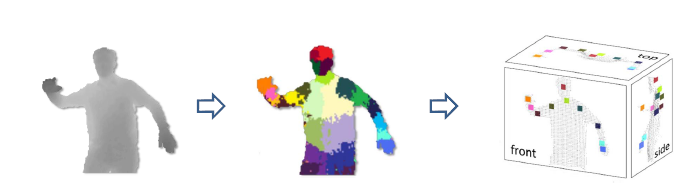
\includegraphics[width=.9\textwidth, keepaspectratio]{fig/kinect-skeleton-algorithm.png}
    \caption{Διαδικασία εξαγωγής της θέσης των αρθρώσεων \cite{shotton11}}
    \label{fig:kinect-skeleton-algorithm}
\end{figure}
%\footnotetext{Σχήμα από την δημοσίευση \cite{shotton11}}

Υπάρχουν δύο υλοποιημένοι αλγόριθμοι ο \eng{body part classification} και ο \eng{offset joint regression}. Θα δώσουμε έμφαση στον πρώτο αλγόριθμο. Αρχικά χρησιμοποιώντας τον χάρτη βάθους για κάθε εικονοστοιχείο υπολογίζεται η συνάρτηση απόστασης \ref{equ:kinect-algorithm-feature-function}, δίνοντας διαφορετικές τιμές στην $\phi$ ώστε να σαρώνεται ο χώρος γύρω από το εικονοστοιχείο που εξετάζεται. Η συνάρτηση απόστασης μπορεί να υπολογιστεί εύκολα και παράλληλα για κάθε εικονοστοιχείο.

\begin{equation}
    f(u|\phi ) = z\big( u + \frac{\delta_1}{z(u)}\big)-z\big( u + \frac{\delta_2}{z(u)}\big)
    \label{equ:kinect-algorithm-feature-function}
\end{equation}

Όπου το $\phi = (\delta_1, \delta_2)$ είναι το χαρακτηριστικό που περιγράφει τις 2\eng{D} μετατοπίσεις από το εικονοστοιχείο \eng{u}, η $z(u)$ δίνει την τιμή βάθους του εικονοστοιχείου. Στην συνέχεια χρησιμοποιώντας τυχαιοποιημένα δέντρα απόφασης (\eng{randomized decision forest}), γίνεται μια ταξινόμηση για τις συγκεκριμένες παραμέτρους $\phi$ και εκτιμάται μια πυκνότητα πιθανότητας, που υποδηλώνει σε ποιο τμήμα του σώματος ανήκει το εικονοστοιχείο. Η διαδικασία επαναλαμβάνεται για όλα τα δέντρα που ανήκουν στο σύνολο και για κάθε εικονοστοιχείο. Τέλος, υπολογίζεται ο μέσος όρος για το συγκεκριμένο εικονοστοιχείο από όλες τις πυκνότητες πιθανότητες που υπολογίστηκαν από κάθε δέντρο απόφασης του συνόλου και ταξινομείται σε ένα τμήμα του σώματος.

\begin{equation}
    p(c|u) = \frac{1}{T} \cdot \sum_{l \in L(u)} p_{l}(c)
    \label{equ:kinect-algorithm-pixel-probability}
\end{equation}

Ως τελικό βήμα με βάση την ταξινόμηση των εικονοστοιχείων του χάρτη βάθους υπολογίζεται η τρισδιάστατη θέση των αρθρώσεων για κάθε τμήμα του σώματος και γίνεται παλινδρόμηση ενός γενικού μοντέλου (σκελετός). Κάτι που δεν αναφέρθηκε είναι ο τρόπος με τον οποίον επιλέγονται οι τιμές $\phi$, που ουσιαστικά είναι μια δειγματοληψία στην γειτονία του εικονοστοιχείου. Επίσης είναι φανερό ότι πρέπει να γίνει μια διαδικασία εκπαίδευσης του αλγορίθμου. Για να επιτευχθεί αυτό αρχικά συλλέχθηκαν εικόνες βάθους για τις οποίες ήταν ήδη γνωστή η θέση των αρθρώσεων οπότε τα εικονοστοιχεία ήταν είδη ταξινομημένα στα αντίστοιχα τμήματα του σώματος. Στη συνέχεια συνθέθηκαν κατάλληλα επιπλέον εικόνες βάθους (Σχήμα \ref{fig:kinect-data-synthesis}) από τις υπάρχουσες με διαφορετικά ανθρωπομετρικά χαρακτηριστικά και διαφορετικούς προσανατολισμούς της κάμερας ώστε να κάνουν τον αλγόριθμο πιο αξιόπιστο και γενικό.

\begin{figure}[H]
    \centering
    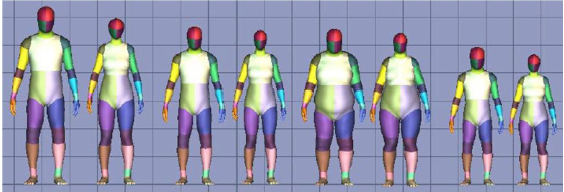
\includegraphics[width=.7\textwidth, keepaspectratio]{fig/kinect-data-synthesis.png}
    \caption{Συνθέσεις των εικόνων βάθους για την εκπαίδευση του αλγορίθμου \cite{shotton11}}
    \label{fig:kinect-data-synthesis}
\end{figure}
%\footnotetext{Σχήμα από την δημοσίευση \cite{shotton11}}

Το πρόβλημα είναι πολύ δύσκολο και εξαρτάται από πολλούς παράγοντες όπως είναι το φως, η διαφοροποίηση των ανθρώπων, οι ποικίλες στάσεις, το χρώμα, το δίσημο και από την παρεμπόδιση τμημάτων του σώματος που δεν είναι ορατά στον αισθητήρα (\eng{occlusion}). Ο αλγόριθμος επιτυγχάνει πολύ υψηλά ποσοστά ανίχνευσης με μεγάλη ακρίβεια. Είναι ταχύτατος, γιατί από την φύση του μπορεί να εκτελεστεί παράλληλα, με αποτέλεσμα η υλοποίηση του να γίνει στο υλικό εσωτερικά και όχι από λογισμικό.

%%%%%%%%%%%%%%%%%%%%%%%%%%%%%%%%%%%%%%%%%%%%%%%%%%%%%%%%%%%%%%%%%%%%%%%%%%%%%%%%
\section{Εργαλεία}

Υπάρχουν πολλές εναλλακτικές λύσεις όσον αφορά το εργαλείο που μπορεί να χρησιμοποιηθεί για πρόσβαση στα δεδομένα που παρέχει το \eng{Kinect}. Παρακάτω αναφέρονται δύο εργαλεία: το προκαθορισμένο \eng{SDK} της \eng{Microsoft} και το εναλλακτικό της \eng{OpenNI}. Και τα δύο είναι εξίσου καλά και χρησιμοποιούνται από πολλούς χρήστες. Τα εργαλεία παρέχουν επιπλέον δυνατότητες για πιο προχωρημένες εφαρμογές όπως είναι η αναγνώριση ομιλίας, αναγνώριση έκφρασης προσώπου, τρισδιάστατη ανακατασκευή και πολλά άλλα. Παρακάτω αναφέρονται κάποια βασικά χαρακτηριστικά και γίνεται μια σύγκριση.

%%%%%%%%%%%%%%%%%%%%%%%%%%%%%%%%%%%%%%%%%%%%%%%%%%%%%%%%%%%%%%%%%%%%%%%%%%%%%%%%
\subsection{\texorpdfstring{Προκαθορισμένο Εργαλείο της \eng{Microsoft}}{}}

\begin{figure}[H]
    \centering
    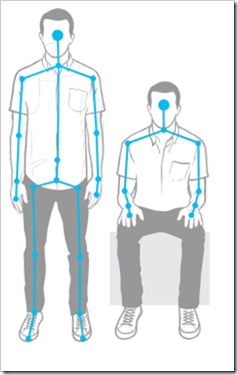
\includegraphics[height=.30\textheight, keepaspectratio]{fig/microsoft-skeleton.png}
    \caption{Σκελετικό σύστημα που παρέχει το εργαλείο της \eng{Microsoft}\protect\footnotemark}
    \label{fig:microsoft-sdk-skeleton}
\end{figure}
\footnotetext{Σχήμα από την ιστοσελίδα \eng{\url{http://msdn.microsoft.com/en-us/library/hh973077.aspx}}}

Το εργαλείο της \eng{Microsoft} είναι δωρεάν και παρέχει πλούσιο ρεπερτόριο από συναρτήσεις για πρόσβαση στην συσκευή. Είναι αποκλειστικά για \eng{Windows} και δεν μπορεί να χρησιμοποιηθεί από αλλά λειτουργικά. Οι γλώσσες προγραμματισμού που χρησιμοποιούνται είναι η \eng{C++} και η \eng{C\#}. Υπάρχει δυνατότητα συνεργασία με άλλες βιβλιοθήκες, όπως είναι η \eng{XNA} και το \eng{DirectX}.

Όσον αφορά την απόκτηση σκελετικής πληροφορίας υπάρχει μια μεγάλη διαφορά στο ότι το \eng{SDK} της \eng{Microsoft} παρέχει πληροφορία 20 αρθρώσεων. Ένα σημαντικό πλεονέκτημα σε σχέση με άλλα εργαλεία είναι ότι δεν απαιτείται βαθμονόμηση του αισθητήρα. Επίσης μπορεί κανείς να ανιχνεύει μέχρι έξι σκελετούς στην ίδια εφαρμογή. Τέλος, παρέχει έτοιμες δομές φίλτρων για την βελτίωση του αποτελέσματος της ακολουθίας των θέσεων, που είναι μια απαραίτητη διαδικασία, αφού υπάρχει πάντα θόρυβος και προβλήματα εκτίμησης της θέσης. Στο Σχήμα \ref{fig:microsoft-sdk-skeleton} φαίνεται ενδεικτικά η δομή του σκελετού που προσφέρεται από το συγκεκριμένο εργαλείο.

%%%%%%%%%%%%%%%%%%%%%%%%%%%%%%%%%%%%%%%%%%%%%%%%%%%%%%%%%%%%%%%%%%%%%%%%%%%%%%%%
\subsection{\texorpdfstring{Εναλλακτικό Εργαλείο της \eng{OpenNI}}{}}

Το εναλλακτικό εργαλείο είναι το \eng{OpenNI}, το οποίο εκτός του \eng{Kinect} δίνει τη δυνατότητα πρόσβασης και σε άλλους αντίστοιχους αισθητήρες με τον ίδιο τρόπο, ενώ έχει μια ξεκάθαρη αρχιτεκτονική που διευκολύνει τον προγραμματιστή (Σχήμα \ref{fig:openni-framework}). Όμοια με το \eng{SDK} της \eng{Microsoft} η \eng{OpenNI} παρέχει πλούσιο ρεπερτόριο από αλγορίθμους και εφαρμογές. Είναι ανοιχτού κώδικα, υπάρχει υλοποίηση τόσο στα \eng{Windows} όσο και στο \eng{Linux} \eng{cross platform}. Οι κύριες γλώσσες προγραμματισμού  που υποστηρίζονται από το \eng{OpenNI} είναι η \eng{C++}, η \eng{Java} και η \eng{Python}.

\begin{figure}[H]
    \centering
    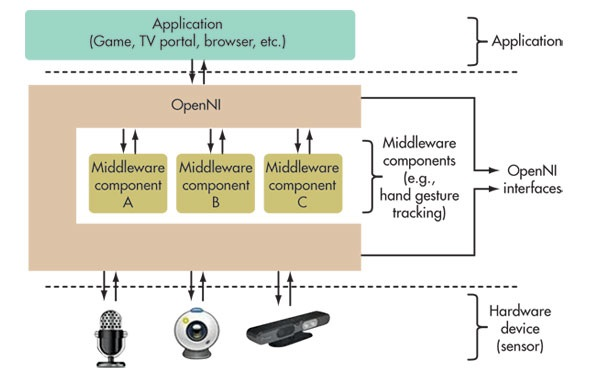
\includegraphics[width=.8\textwidth, height=.3\textheight, keepaspectratio]{fig/openni-framework.jpg}
    \caption{Αρχιτεκτονική της βιβλιοθήκης της \eng{OpenNI}\protect\footnotemark}
    \label{fig:openni-framework}
\end{figure}
\footnotetext{Σχήμα από την ιστοσελίδα \eng{\url{http://electronicdesign.com/embedded/how-microsoft-s-primesense-based-kinect-really-works}}}

\begin{figure}[H]
    \centering
    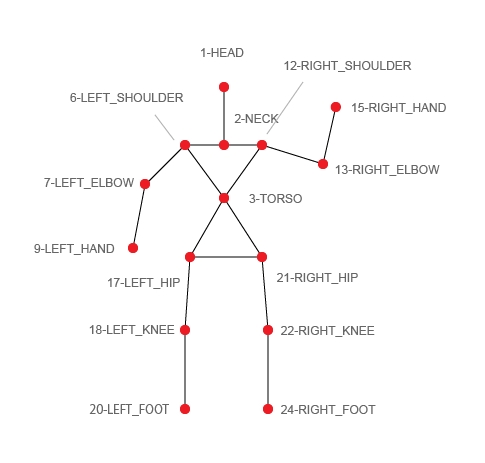
\includegraphics[width=.7\textwidth, height=.35\textheight, keepaspectratio]{fig/openni-skeleton.png}
    \caption{Σκελετικό σύστημα που προσφέρει το εργαλείο της \eng{OpenNI}}
    \label{fig:openni-skeleton}
\end{figure}

Όσον αφορά την εξαγωγή του σκελετού, μειονεκτεί σε σύγκριση με το αντίστοιχο εργαλείο της \eng{Microsoft}. Αυτό γιατί παρέχει 16 αρθρώσεις όπως φαίνεται στο Σχήμα \ref{fig:openni-skeleton}, που ίσως δεν είναι αρκετές για την εφαρμογή, ειδάλλως δεν είναι τόσο κρίσιμη διαφορά. Ένα βασικό μειονέκτημα είναι η απαίτηση βαθμονόμησης της συσκευής. Επίσης σημαντικό είναι το κομμάτι που αφορά την βελτίωση των μετρήσεων, καθώς το \eng{OpenNI} δεν παρέχει έτοιμες δομές, κάτι που χρειάζεται χρόνο για να υλοποιηθεί. Για τους παραπάνω λόγους προτιμήθηκε το εργαλείο της \eng{Microsoft}. Ενδεικτικά στον Πίνακα \ref{tab:openni-microsoft} φαίνονται κάποιες βασικές διαφορές.

\begin{center}
    \begin{tabular}{lcc}
        \toprule
        % after \\: \hline or \cline{col1-col2} \cline{col3-col4} ...
        \multicolumn{1}{c}{Χαρακτηριστικά} & \eng{OpenNI} & \eng{Microsoft SDK} \\
        \midrule
        Πρόσβαση στα δεδομένα βάθους και \eng{RGB} & Ναι & Ναι \\
        Ανίχνευση αρθρώσεων & Ναι & Ναι \\
        Υποστήριξη αναγνώρισης χειρονομιών & Ναι & Όχι \\
        Συναρτήσεις άμεσης αποθήκευσης δεδομένων στο δίσκο & Ναι & Όχι \\
        Βαθμονόμιση & Ναι & Όχι \\
        Υποστήριξη επεξεργασίας ήχου και αναγνώριση ομιλίας & Όχι & Ναι \\
        Ευκολία εγκατάστασης & Όχι & Ναι \\
        Διαθέσιμος αριθμός αρθρώσεων & 16 & 20 \\
        Ποιότητα εγχειριδίων τεκμηρίωσης  & Καλή & Μέτρια\\
        \bottomrule
    \end{tabular}
    \captionof{table}{Σύγκριση βασικών χαρακτηριστικών μεταξύ των δύο εργαλείων}
    \label{tab:openni-microsoft}
\end{center}

\vfil

%%%%%%%%%%%%%%%%%%%%%%%%%%%%%%%%%%%%%%%%%%%%%%%%%%%%%%%%%%%%%%%%%%%%%%%%%%%%%%%%
\section{Σύστημα Μετρήσεων}

Η συλλογή ορθών μετρήσεων είναι ένα σημαντικό βήμα για την εξαγωγή σωστών αποτελεσμάτων στα μετέπειτα στάδια. Η καταγραφή της βάδισης του ανθρώπου είναι η βάση για πολλές αναλύσεις από τις οποίες μπορούν να εξαχθούν χρήσιμα αποτελέσματα. Ενδεικτικά θα ήταν χρήσιμη η μελέτη της δυναμικής συμπεριφοράς του σώματος κατά την διεξαγωγή μιας κίνησης, ώστε να μπορεί να μελετηθεί η συμπεριφορά του μυοσκελετικού συστήματος. Πρέπει να δοθεί μεγάλη βαρύτητα στην απόκτηση έγκυρων μετρήσεων και για το λόγο αυτό απαιτείται η δημιουργία αλγορίθμων που θα ελαχιστοποιούν τα σφάλματα και θα διώχνουν τον θόρυβο. Στην συνέχεια εξηγούμε κάποια ενδεικτικά προβλήματα κατά την διαδικασία της καταγραφής και την αντιμετώπιση τους.

%%%%%%%%%%%%%%%%%%%%%%%%%%%%%%%%%%%%%%%%%%%%%%%%%%%%%%%%%%%%%%%%%%%%%%%%%%%%%%%%
\subsection{Τροχιές των Αρθρώσεων}

Ο προγραμματιστής  μπορεί να έχει πρόσβαση στα δεδομένα της συσκευής που αφορούν τις συντεταγμένες των αρθρώσεων. Δεδομένου ότι έχει ενεργοποιηθεί εσωτερικά (από τον προγραμματιστή) η ανίχνευση του σκελετού και στο πεδίο ορατότητας της συσκευής έχει ανιχνευθεί αντικείμενο ανθρώπινης μορφής, τότε η συσκευή στέλνει πακέτα με την πληροφορία των θέσεων των αρθρώσεων πίσω στον χρήστη. Το πακέτο περιέχει επιπλέον πληροφορίες για τις αρθρώσεις, όπως είναι ο προσανατολισμός (προϋποθέτει ιεραρχική δομή σκελετού), σκορ εμπιστοσύνης για την μέτρηση (που κυμαίνεται από 0 έως 1) και κάποιες ενδείξεις αν έχει εξαχθεί συμπέρασμα για την θέση της άρθρωσης. Στην ανάλυση το ενδιαφέρον εστιάζεται στη θέση με την πάροδο του χρόνου. Έστω ότι έχουμε $Ν$ αριθμό αρθρώσεων που αποθηκεύονται σε συγκεκριμένες χρονικές στιγμές.

\begin{equation}
    p^{t}_{j} = \{x^{t}_{j}, y^{t}_{j}, z^{t}_{j}\}, \quad t \in (0, t), \quad j \in (0, N)
    \label{equ:trajectories}
\end{equation}

Όπου \eng{p} είναι η Καρτεσιανή θέση την χρονική στιγμή \eng{t} για την άρθρωση \eng{j}. Η αρχή των αξόνων είναι η θέση του \eng{Kinect} και ο άξονας \eng{Z} είναι το βάθος όπως φαίνεται στο Σχήμα \ref{fig:kinect-joints}.

Πρέπει να διευκρινιστεί ότι τα δεδομένα δεν έρχονται περιοδικά σε ντετερμινιστικές χρονικές στιγμές, αλλά έχουν μια απόκλιση που οφείλεται κυρίως στο \eng{software} και στις εσωτερικές καθυστερήσεις, αλλά και σε επίπεδο υλικού. Για το λόγο αυτό είναι χρήσιμο να γίνει η μέτρηση της χρονικής στιγμής που έρχονται και αποθηκεύονται τα δεδομένα ώστε να χρησιμοποιηθεί στα μετέπειτα στάδια της ανάλυσης. Μια άλλη παρατήρηση είναι ότι τα δεδομένα βρίσκονται στο σύστημα συντεταγμένων με αρχή των αξόνων το \eng{Kinect} και ανάλογα το εργαλείο που θα χρησιμοποιηθεί στα μετέπειτα στάδια της επεξεργασίας θα πρέπει να γίνει η κατάλληλη μετατροπή συστήματος συντεταγμένων.

\begin{figure}[H]
    \centering
    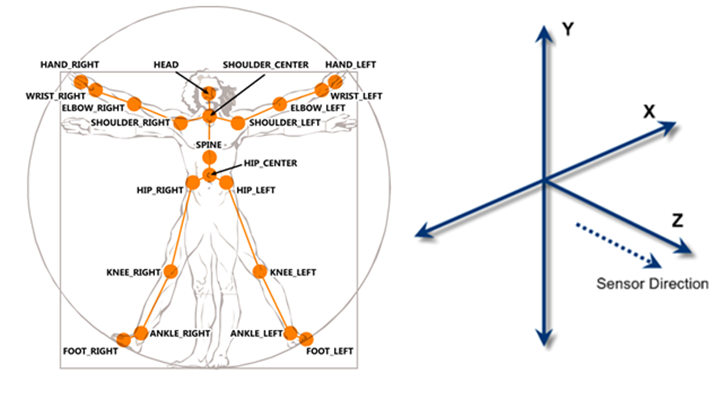
\includegraphics[width=.9\textwidth, keepaspectratio]{fig/kinect-joints.png}
    \caption{Το σύστημα αρθρώσεων που χρησιμοποιήθηκε\protect\footnotemark}
    \label{fig:kinect-joints}
\end{figure}
\footnotetext{Σχήμα από την ιστοσελίδα \eng{\url{http://msdn.microsoft.com/en-us/library/jj131025.aspx}}}

%%%%%%%%%%%%%%%%%%%%%%%%%%%%%%%%%%%%%%%%%%%%%%%%%%%%%%%%%%%%%%%%%%%%%%%%%%%%%%%%
\subsection{Αντιμετώπιση του Θορύβου}

Υπάρχουν πολλά ενοχλητικά προβλήματα που εμφανίζονται στην πράξη και καθιστούν τις μετρήσεις \lq μην κατάλληλες\rq\: για επεξεργασία. Ο θόρυβος επηρεάζεται από πολλούς παράγοντες, όπως είναι ο φωτισμός στον χώρο που διεξάγεται το πείραμα, η στάση του σώματος, η τοποθεσία της συσκευής και πολλά άλλα. Ένα πολύ εμφανές παράδειγμα θορύβου εμφανίζεται κατά την εκτίμηση της θέσης της άρθρωσης, λόγω της μικρής απόκλισης της τιμής από την προηγούμενη μέτρηση, με αποτέλεσμα να δίνει την αίσθηση ότι το δείγμα τρέμει ενώ στην πραγματικότητα είναι στάσιμο όπως φαίνεται και στο Σχήμα \ref{fig:hand2}.

Για την αντιμετώπιση του προβλήματος μπορούν να υλοποιηθούν απλές τεχνικές φιλτραρίσματος και να ελαχιστοποιηθεί ο θόρυβος. Πρέπει κανείς να ξεχωρίσει κάποια κριτήρια που είναι το ποσοστό της εξομάλυνσης των πολύ απότομων κινήσεων, την καθυστέρηση που εισάγεται από την αλλαγή που προκαλεί η φάση του φίλτρου και το αν η εφαρμογή είναι πραγματικού χρόνου (\eng{online}) ή μη (\eng{offline}).

Αν επιλεχθεί να αποκοπούν οι ψηλές συχνότητες (απότομες κινήσεις), τότε θα αντιμετωπιστεί το πρόβλημα που αναφέρεται πιο πάνω και το αποτέλεσμα θα είναι αυτό του Σχήματος \ref{fig:hand1}. Ο θόρυβος αυτής της μορφής στην ξένη βιβλιογραφία αναφέρεται σαν \lq \eng{jitter}\rq . Πρέπει ωστόσο να δοθεί προσοχή διότι το σύστημα θα αγνοεί πέραν του θορύβου και τις απότομες κινήσεις του δείγματος, κάτι που ίσως είναι ανεπιθύμητο. Η σωστή επιλογή αυτών των παραμέτρων είναι κρίσιμη και εξαρτάται από την εφαρμογή που μας ενδιαφέρει και κυρίως από την ταχύτητα του δείγματος.

\begin{figure}[H]
    \centering
    \begin{subfigure}[t]{.4\textwidth}
        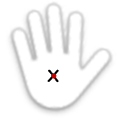
\includegraphics[width=.7\textwidth, keepaspectratio]{fig/hand1.png}
        \caption{Βέλτιστη εκτίμηση της θέσης του χεριού}
        \label{fig:hand1}
    \end{subfigure}
    \begin{subfigure}[t]{.4\textwidth}
        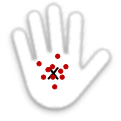
\includegraphics[width=.7\textwidth, keepaspectratio]{fig/hand2.png}
        \caption{Αβεβαιότητα στον προσδιορισμό της θέσης}
        \label{fig:hand2}
    \end{subfigure}
    \caption{Πρόβλημα εκτίμησης θέσης λόγω του θορύβου \eng{jitter}\protect\footnotemark}
\end{figure}
\footnotetext{Σχήμα από την ιστοσελίδα \eng{\url{http://msdn.microsoft.com/en-us/library/jj131429.aspx}}}

Όπως φαίνεται στο Σχήμα \ref{fig:filter-latency} με κόκκινο είναι η τροχιά, όπου βλέπουμε τις ανεπιθύμητες μεταβολές λόγω θορύβου. Με μπλε χρώμα απεικονίζεται η τροχιά μετά το φιλτράρισμα, όπου παρατηρούμε ότι έχει εξομαλυνθεί ο θόρυβος, αλλά έχει δημιουργηθεί καθυστέρηση των δειγμάτων. Κάτι που αξίζει να σημειωθεί είναι ότι αν η εφαρμογή δεν απαιτείται να είναι πραγματικού χρόνου, τότε μπορούν να χρησιμοποιηθούν μην αιτιατά φίλτρα, που λαμβάνουν υπόψη στους υπολογισμούς τις μελλοντικές τιμές, με αποτέλεσμα να γίνει καλύτερη εκτίμηση της τροχιάς.

Για παράδειγμα μια απλή τεχνική για την αφαίρεση του θορύβου λόγω \eng{jitter} βασίζεται στην απλή σχέση αναδρομής \ref{equ:jitter-removal}.

\begin{equation}
    \hat{p}_{n} =
    \begin{cases}
        p_{n}, & \text{Αν } \|p_{n} - \hat{p}_{n-1}\| < \text{κατώφλι} \\
        a \cdot p_{n} + (1-a) \cdot \hat{p}_{n-1}, & \text{αλλιώς}
    \end{cases}
    \label{equ:jitter-removal}
\end{equation}

Μια κατηγορία από φίλτρα που μπορούν να χρησιμοποιηθούν είναι τα παρακάτω:

\begin{itemize}
    \item Κινούμενος μέσος όρος (χαμηλοπερατό)
    \item \eng{Savitzky–Golay} (ελαχιστοποιεί το τετραγωνικό σφάλμα)
    \item \eng{Exponential Smoothing Filter} (εκθετικό βάρος στις μετρήσεις)
    \item \eng{Adaptive Double Exponential Smoothing Filter} (πρόβλεψη και μεταβολή των συντελεστών)
    \item \eng{Taylor Series} (δεν έχει μεγάλο παράθυρο πρόβλεψης)
    \item \eng{Median Filter} (απαλοιφή θόρυβος)
\end{itemize}

\begin{figure}[H]
    \centering
    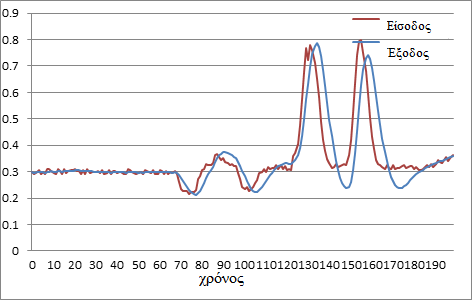
\includegraphics[width=.8\textwidth, keepaspectratio]{fig/filter-latency.png}
    \caption{Εξομάλυνση και καθυστέρηση της ακολουθίας μετά το φιλτράρισμα\protect\footnotemark}
    \label{fig:filter-latency}
\end{figure}
\footnotetext{Σχήμα από την ιστοσελίδα \eng{\url{http://msdn.microsoft.com/en-us/library/jj131429.aspx}}}

Από τα παραπάνω φίλτρα ο κινούμενος μέσος όρος ουσιαστικά εξομαλύνει το αποτέλεσμα αλλά δεν έχει μεγάλες δυνατότητες πρόβλεψης. Σε αντίθεση τα φίλτρα \eng{Savitzky–Golay} εκτελούν παλινδρόμηση με χρήση πολυωνύμων, ελαχιστοποιώντας το τετραγωνικό σφάλμα και κατόπιν κάνουν πρόβλεψη για την επόμενη χρονική στιγμή με βάση το πολυώνυμο που έχει εκτιμηθεί. Τα \eng{Exponential Smoothing Filter} εξομαλύνουν το αποτέλεσμα λαμβάνοντας υπόψιν τις $Κ$ χρονικές στιγμές, με βάρη που φθίνουν εκθετικά, δίνοντας λιγότερη βαρύτητα σε παλαιότερες μετρήσεις. Τα \eng{Adaptive Double Exponential Smoothing} φίλτρα κάνουν ένα είδος πρόβλεψης με χρήση της ταχύτητας και παράλληλα χρησιμοποιούν συντελεστές βαρύτητας οι όποιοι μεταβάλλονται κατάλληλα και ακολουθούν την εξής αναδρομική σχέση \ref{equ:double-exponential}. Οι σειρές \eng{Taylor} προσεγγίζουν ένα πολυώνυμο με χρήση των παραγώγων και έπειτα προβλέπουν την επόμενη χρονική θέση με βάση αυτό. Οι σειρές \eng{Taylor} δεν έχουν μεγάλο παράθυρο πρόβλεψης. Τέλος, υπάρχουν απλές υλοποιήσεις φίλτρων για την απαλοιφή του θορύβου όπως είναι το \eng{Median} φίλτρο. Στον Πίνακα \ref{tab:filter-parameters} αναφέρονται οι παράμετροι που χρησιμοποιήθηκαν, ανάλογα με την εφαρμογή, ενώ για το επιθυμητό αποτέλεσμα του φιλτραρίσματος μπορούν να επιλεχθούν κατάλληλες τιμές ως παράμετροι των φίλτρων. Οι τιμές αυτές εκτιμήθηκαν πειραματικά με κριτήριο την ταχύτητα απόκρισης αλλά και την καθαρότητα της καταγεγραμμένης κίνησης.

\begin{equation}
    \begin{aligned}
        b_{n} = \gamma \cdot (\hat{p}_{n} - \hat{p}_{n-1}) + (1 - \gamma) \cdot b_{n-1}\\[10pt]
        \hat{p}_{n} = \alpha \cdot p_{n} + (1 - a) \cdot (\hat{p}_{n-1} + b_{n-1})
    \end{aligned}
    \label{equ:double-exponential}
\end{equation}

\vspace{10pt}

\begin{center}
    \begin{threeparttable}
        \begin{tabular}{lccc}
            \toprule
            % after \\: \hline or \cline{col1-col2} \cline{col3-col4} ...
            Παράμετροι & Κανονικό\tnote{α} & Μέτριο\tnote{β} & Δυνατό\tnote{γ} \\
            \midrule
            Εξομάλυνση & 0.5 & 0.5 & 0.7 \\
            Διόρθωση & 0.5 & 0.1 & 0.3 \\
            Πρόβλεψη & 0.5 & 0.5 & 1.0 \\
            Ακτίνα θορύβου & 0.05 & 0.1 & 1.0 \\
            Μέγιστη απόκλιση & 0.04 & 0.1 & 1.0 \\
            \bottomrule
        \end{tabular}
        \begin{tablenotes}
            \item[α] Φιλτράρει ελαφρώς το \eng{jitter}. Καλό για εφαρμογές αναγνώρισης σε παιχνίδια, όπου υπάρχουν απότομες κινήσεις.
            \item[β] Μειώνει αρκετά το \eng{jitter}. Είναι καλό για εφαρμογές όπου απαιτείται ομαλή κίνηση.
            \item[γ] Μειώνει πολύ το \eng{jitter}. Αφορά εφαρμογές που δεν ενδιαφερόμαστε για την καθυστέρηση της κίνησης.
        \end{tablenotes}
    \end{threeparttable}
    \captionof{table}{Ενδεικτικές παράμετροι των φίλτρων της \eng{Microsoft} που χρησιμοποιήθηκαν}
    \label{tab:filter-parameters}
\end{center}

%\begin{itemize}
%	\item \eng{Smoothing} παράμετρος εξομάλυνσης
%	\item \eng{Correction} μικρές τιμές τείνουν να μοιάζουν με τα δεδομένα που έχουμε
%	\item \eng{Prediction} συμβολίζει την εκτίμηση που κάνουμε για μελλοντικές τιμές
%	\item \eng{JitterRadius} η ακτίνα σε μέτρα για την μείωση του \eng{jitter}
%    \item \eng{MaxDeviationRadius} η μέγιστη διασπορά στην ακτίνα την οποία μπορεί να ανεχτεί το φίλτρο
%\end{itemize}

